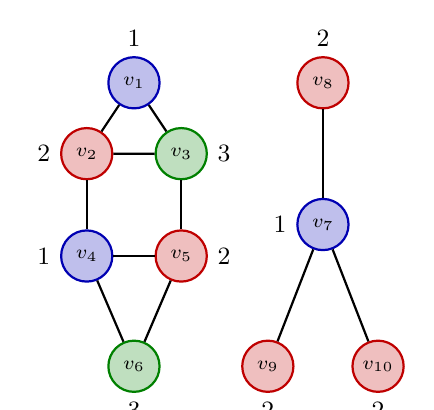
\begin{tikzpicture}[
  baseline=0pt,
  scale=1,
  vnode/.style={circle, draw=black, fill=blue!20, thick, inner sep=0pt, minimum size=6.5mm},
  edge/.style={thick, draw=black},
  clabel/.style={font=\small, color=black},
  % Colores de la coloración (los mismos de las flechas de la Tabla)
  col1/.style={fill=blue!70!black!25, draw=blue!70!black},
  col2/.style={fill=red!75!black!25, draw=red!75!black},
  col3/.style={fill=green!50!black!25, draw=green!50!black},
  col4/.style={fill=orange!90!black!25, draw=orange!90!black}
]
  % Se amplía xmin a -2.55 para añadir el medio carácter de margen izquierdo
  \useasboundingbox (-2.55,-2.2) rectangle (2.25,2.3);

  \begin{scope}[yshift=-0.2cm]
    % --- COMPONENTE 1 ---
    \node[vnode, col1, label={[clabel]above:$1$}] (v1) at (-1.2, 1.8) {$\scriptstyle v_1$};
    \node[vnode, col2, label={[clabel]left:$2$}]  (v2) at (-1.8, 0.9) {$\scriptstyle v_2$};
    \node[vnode, col3, label={[clabel]right:$3$}] (v3) at (-0.6, 0.9) {$\scriptstyle v_3$};
    \node[vnode, col1, label={[clabel]left:$1$}]  (v4) at (-1.8, -0.4) {$\scriptstyle v_4$};
    \node[vnode, col2, label={[clabel]right:$2$}] (v5) at (-0.6, -0.4) {$\scriptstyle v_5$};
    \node[vnode, col3, label={[clabel]below:$3$}] (v6) at (-1.2, -1.8) {$\scriptstyle v_6$};

    \draw[edge] (v1) -- (v2) -- (v3) -- (v1);
    \draw[edge] (v2) -- (v4);
    \draw[edge] (v3) -- (v5);
    \draw[edge] (v4) -- (v5);
    \draw[edge] (v4) -- (v6);
    \draw[edge] (v5) -- (v6);

    % --- COMPONENTE 2 ---
    \node[vnode, col1, label={[clabel]left:$1$}]  (v7)  at (1.2, 0.0) {$\scriptstyle v_7$};
    \node[vnode, col2, label={[clabel]above:$2$}] (v8)  at (1.2, 1.8) {$\scriptstyle v_8$};
    \node[vnode, col2, label={[clabel]below:$2$}] (v9)  at (0.5, -1.8) {$\scriptstyle v_9$};
    \node[vnode, col2, label={[clabel]below:$2$}] (v10) at (1.9, -1.8) {$\scriptstyle v_{10}$};

    \draw[edge] (v7) -- (v8);
    \draw[edge] (v7) -- (v9);
    \draw[edge] (v7) -- (v10);
  \end{scope}
\end{tikzpicture}
